% answers.tex —— 1982 年·全国卷（文科） · 参考答案与详细解析片段
% 由 tools/generate_projects.py 依来源总账自 1982/1982_数学真题_文_试题.md + 1982/1982_数学真题_文_解析正文.md + 1982/1982_数学真题_文_答案要点.md 生成，勿手改（改源 MD 后重跑）


\begin{gknotice}
\textbf{解析归属}：本卷仅题面、无答案页。下列解析由本库逐题独立推导并复算，不声称代表官方发布的标准答案。

\textbf{编注}：第 5 题的篱笆总长按原卷配图理解——图中隔篱垂直于墙，即“平行于一边的篱笆”指的是平行于\textbf{垂直于墙的那两条边}，故隔篱长度为场地之“宽”。若把隔篱读作平行于墙，则篱笆总长为 $2x+2y=L$，最大面积为 $L^2/16$，与图不符；本文按图形取 $x+3y=L$。

\textbf{编注}：第 9 题原卷配图为示意图，其比例（图中 $OA$ 画得比 $OB$ 长）与题设 $a\ge b$ 并不一致；本文按题设条件重绘，仍保持原卷布局（$OB$ 竖直、三条垂线 $AB_1$、$A_1B_2$、$A_2B_3$ 画成水平线）。
\end{gknotice}

\begin{answer}
\gksolhead{1}{}

\textbf{题目}：

填表：

\begin{center}
\begin{tabular}{cll}
\toprule
 & 函数 & 使函数有意义的 $x$ 的实数范围 \\
\midrule
1 & $y=\sqrt{-x^2}$ &  \\
2 & $y=\sqrt{(-x)^2}$ &  \\
3 & $y=10^{\lg x}$ &  \\
4 & $y=\lg 10^x$ &  \\
\bottomrule
\end{tabular}
\end{center}

\Needspace{4\baselineskip}
\textbf{解析}

逐行求使根式（或对数式）有意义的 $x$ 范围。

\Needspace{5\baselineskip}
1. $y=\sqrt{-x^2}$。被开方式须非负：$-x^2\ge0$，即 $x^2\le0$。因 $x^2\ge0$ 恒成立，故只能 $x^2=0$，即
\nopagebreak[4]
\[
x=0.
\]
此时 $y=\sqrt0=0$ 有意义；$x\ne0$ 时被开方式为负，无实义。

\Needspace{5\baselineskip}
2. $y=\sqrt{(-x)^2}$。被开方式 $(-x)^2=x^2\ge0$ 对一切实数成立，根式恒有意义，故
\nopagebreak[4]
\[
x\in\mathbf{R}\quad(\text{全体实数}).
\]
（此时 $y=\sqrt{x^2}=\lvert x\rvert$。）

\Needspace{5\baselineskip}
3. $y=10^{\lg x}$。式中 $\lg x$ 要求真数为正，即
\nopagebreak[4]
\[
x>0.
\]
当 $x>0$ 时 $\lg x$ 为实数，$10^{\lg x}=x$ 有意义；$x\le0$ 时 $\lg x$ 无实义。

\Needspace{5\baselineskip}
4. $y=\lg 10^x$。因对一切实数 $x$ 都有 $10^x>0$，对数真数恒正，故
\nopagebreak[4]
\[
x\in\mathbf{R}\quad(\text{全体实数}).
\]
（此时 $\lg 10^x=x$。）

复算：取 $x=0$ 代入第 1 行得 $y=\sqrt0=0$ ，取 $x=1$ 得 $y=\sqrt{-1}$ 无实义 ；第 2 行取 $x=-3$ 得 $y=\sqrt9=3$ ；第 3 行取 $x=100$ 得 $10^{\lg100}=10^2=100$ ，取 $x=-1$ 时 $\lg(-1)$ 无实义 ；第 4 行取 $x=-2$ 得 $\lg 10^{-2}=-2$ 。

\gkanswer{答案：逐行依次为 $x=0$；全体实数 $\mathbf{R}$；$x>0$；全体实数 $\mathbf{R}$}

\end{answer}
\begin{answer}
\gksolhead{2}{}

\textbf{题目}：

求 $(-1+\mathrm i)^{20}$ 展开式中第 15 项的数值。

\Needspace{4\baselineskip}
\textbf{解析}

\Needspace{5\baselineskip}
把 $(-1+\mathrm i)^{20}$ 看作二项展开式，第 $k$ 项（按展开顺序第 $k$ 项，$1\le k\le21$）为
\nopagebreak[4]
\[
T_k=\mathrm C_{20}^{k-1}(-1)^{21-k}\mathrm i^{\,k-1}.
\]
\Needspace{5\baselineskip}
取 $k=15$：
\nopagebreak[4]
\[
T_{15}=\mathrm C_{20}^{14}(-1)^{6}\mathrm i^{14}.
\]
\Needspace{5\baselineskip}
由 $\mathrm C_{20}^{14}=\mathrm C_{20}^{6}$，
\nopagebreak[4]
\[
\mathrm C_{20}^{6}=\frac{20\cdot19\cdot18\cdot17\cdot16\cdot15}{6!}=\frac{27907200}{720}=38760.
\]
\Needspace{5\baselineskip}
又 $(-1)^6=1$，且
\nopagebreak[4]
\[
\mathrm i^{14}=(\mathrm i^4)^3\cdot\mathrm i^2=1^3\cdot(-1)=-1,
\]
\Needspace{5\baselineskip}
故
\nopagebreak[4]
\[
T_{15}=38760\times1\times(-1)=-38760.
\]

复算（用通项直接展开核对）：逐项算出 $j=0,1,\dots,20$ 的 $\mathrm C_{20}^{j}(-1)^{20-j}\mathrm i^{j}$，第 $j=14$ 项（即第 $15$ 项）为 $-38760$；且全部 $21$ 项之和恰为 $(-1+\mathrm i)^{20}$。又由 $(-1+\mathrm i)=-1\cdot(1-\mathrm i)$ 得 $(-1+\mathrm i)^{20}=(1-\mathrm i)^{20}=\left[(1-\mathrm i)^2\right]^{10}=(-2\mathrm i)^{10}=2^{10}\mathrm i^{10}=-1024$，与逐项求和所得 $-1024$ 一致 。

\gkanswer{答案：$-38760$}

\end{answer}
\begin{answer}
\gksolhead{3}{}

\textbf{题目}：

在平面直角坐标系内，表中的方程表示什么曲线？并画出它们的图形：

\begin{center}
\begin{tabular}{clll}
\toprule
 & 方程 & 曲线名称 & 图形 \\
\midrule
1 & $4x^2+y^2=4$ &  &  \\
2 & $x-3=0$ &  &  \\
\bottomrule
\end{tabular}
\end{center}

\Needspace{4\baselineskip}
\textbf{解析}

\Needspace{5\baselineskip}
1. 方程 $4x^2+y^2=4$ 两边除以 $4$：
\nopagebreak[4]
\[
\frac{x^2}{1}+\frac{y^2}{4}=1.
\]
这是\textbf{椭圆}的标准方程，中心在原点，长轴在 $y$ 轴上：$x$ 方向半轴长 $1$，$y$ 方向半轴长 $2$；顶点为 $(\pm1,0)$ 与 $(0,\pm2)$，焦点为 $(0,\pm\sqrt3)$。
作图：在坐标系中描出四个顶点，连成中心在原点的扁长椭圆（左右窄、上下长）。

2. 方程 $x-3=0$ 即 $x=3$，表示\textbf{一条直线}：它垂直于 $x$ 轴（平行于 $y$ 轴），且过点 $(3,0)$。
作图：在 $x$ 轴上取点 $3$，作过该点的竖直线。

复算：把 $(1,0)$ 代入 $4x^2+y^2=4$ 得 $4=4$ ，$(0,2)$ 得 $4=4$ ，而 $(1,1)$ 得 $5\ne4$ （点确在椭圆上、内部/外部关系正确）；直线 $x=3$ 上任取两点 $(3,0)$、$(3,5)$ 均满足方程 。

\gkanswer{答案：$4x^2+y^2=4$ 表示椭圆 $\dfrac{x^2}{1}+\dfrac{y^2}{4}=1$（中心在原点，长轴在 $y$ 轴上，顶点为 $(\pm1,0)$、$(0,\pm2)$）；$x-3=0$ 表示垂直于 $x$ 轴且过点 $(3,0)$ 的直线}

\end{answer}
\begin{answer}
\gksolhead{4}{}

\textbf{题目}：

已知 $x-y=\dfrac12$，$x^2+y^2=1$，求 $x^2-y^2$ 的值。

\Needspace{4\baselineskip}
\textbf{解析}

\Needspace{5\baselineskip}
由 $x-y=\dfrac12$ 平方：
\nopagebreak[4]
\[
x^2-2xy+y^2=\frac14.
\]
\Needspace{5\baselineskip}
又已知 $x^2+y^2=1$，代入得
\nopagebreak[4]
\[
1-2xy=\frac14\ \Longrightarrow\ 2xy=\frac34\ \Longrightarrow\ xy=\frac38.
\]
\Needspace{5\baselineskip}
于是
\nopagebreak[4]
\[
(x+y)^2=x^2+y^2+2xy=1+\frac34=\frac74,
\]
\Needspace{5\baselineskip}
故
\nopagebreak[4]
\[
x+y=\pm\frac{\sqrt7}{2}.
\]
\Needspace{5\baselineskip}
所求
\nopagebreak[4]
\[
x^2-y^2=(x-y)(x+y)=\frac12\times\left(\pm\frac{\sqrt7}{2}\right)=\pm\frac{\sqrt7}{4}.
\]

\Needspace{5\baselineskip}
两个符号都确有其解：解方程组 $\begin{cases}x-y=\frac12\\ xy=\frac38\end{cases}$，即 $x$、$y$ 是 $u^2-su+\frac38=0$（$s=x+y$）的两根，其判别式
\nopagebreak[4]
\[
s^2-4\cdot\frac38=\frac74-\frac32=\frac14>0,
\]
两解均为实数。

复算：取 $x+y=\dfrac{\sqrt7}{2}\approx1.32288$，则 $x\approx0.91144$、$y\approx0.41144$，得 $x-y\approx0.5$ 、$x^2+y^2\approx0.83072+0.16928=1$ 、$x^2-y^2\approx0.66144=\dfrac{\sqrt7}{4}$ ；取 $x+y=-\dfrac{\sqrt7}{2}$ 时 $x\approx-0.41144$、$y\approx-0.91144$，同样满足两条件而 $x^2-y^2\approx-0.66144$ 。

\gkanswer{答案：$\pm\dfrac{\sqrt7}{4}$}

\end{answer}
\begin{answer}
\gksolhead{5}{}

\textbf{题目}：

以墙为一边，用篱笆围成长方形的场地，并用平行于一边的篱笆隔开（如图）。已知篱笆的总长为定值 $L$，这块场地的长和宽各为多少时场地的面积最大？最大面积是多少？
\nopagebreak[4]
\begin{center}% 1982 年全国卷（文科）第 5 题：以墙为一边、用篱笆围长方形场地，并以平行于宽边的篱笆隔成两块；上沿为带砖缝与短刻线的墙，墙两端略长于场地，左块窄、右块宽（按源卷布局）
\begin{tikzpicture}[scale=1, line width=0.5pt,
  every node/.style={inner sep=1.5pt}]
  % 墙：上沿 y=4.00、下沿 y=3.60 两条水平线
  \draw (0,4.00) -- (8,4.00);
  \draw (0,3.60) -- (8,3.60);
  % 砖缝（两线之间）
  \foreach \x in {0.65,1.45,2.25,3.05,3.85,4.65,5.45,6.25,7.05,7.85} {
    \draw (\x,3.60) -- (\x,4.00);
  }
  % 上沿短刻线
  \foreach \x in {0.25,1.05,1.85,2.65,3.45,4.25,5.05,5.85,6.65,7.45} {
    \draw (\x,4.00) -- (\x,4.27);
  }
  % 下沿短刻线
  \foreach \x in {0.25,1.05,1.85,2.65,3.45,4.25,5.05,5.85,6.65,7.45} {
    \draw (\x,3.60) -- (\x,3.33);
  }
  % 场地：左篱、中隔篱（平行于两侧的篱笆）、右篱均上端接墙的下沿，另加下横篱
  \draw (1.00,3.60) -- (1.00,0.38);
  \draw (2.95,3.60) -- (2.95,0.38);
  \draw (6.90,3.60) -- (6.90,0.38);
  \draw (1.00,0.38) -- (6.90,0.38);
\end{tikzpicture}
\end{center}
\nopagebreak[4]
\Needspace{4\baselineskip}
\textbf{解析}
\nopagebreak[4]
\begin{center}% 1982 年全国卷（文科）第 5 题：以墙为一边、用篱笆围长方形场地，并以平行于宽边的篱笆隔成两块；上沿为带砖缝与短刻线的墙，墙两端略长于场地，左块窄、右块宽（按源卷布局）
\begin{tikzpicture}[scale=1, line width=0.5pt,
  every node/.style={inner sep=1.5pt}]
  % 墙：上沿 y=4.00、下沿 y=3.60 两条水平线
  \draw (0,4.00) -- (8,4.00);
  \draw (0,3.60) -- (8,3.60);
  % 砖缝（两线之间）
  \foreach \x in {0.65,1.45,2.25,3.05,3.85,4.65,5.45,6.25,7.05,7.85} {
    \draw (\x,3.60) -- (\x,4.00);
  }
  % 上沿短刻线
  \foreach \x in {0.25,1.05,1.85,2.65,3.45,4.25,5.05,5.85,6.65,7.45} {
    \draw (\x,4.00) -- (\x,4.27);
  }
  % 下沿短刻线
  \foreach \x in {0.25,1.05,1.85,2.65,3.45,4.25,5.05,5.85,6.65,7.45} {
    \draw (\x,3.60) -- (\x,3.33);
  }
  % 场地：左篱、中隔篱（平行于两侧的篱笆）、右篱均上端接墙的下沿，另加下横篱
  \draw (1.00,3.60) -- (1.00,0.38);
  \draw (2.95,3.60) -- (2.95,0.38);
  \draw (6.90,3.60) -- (6.90,0.38);
  \draw (1.00,0.38) -- (6.90,0.38);
\end{tikzpicture}
\end{center}
\nopagebreak[4]
设场地平行于墙的一边（长）为 $x$，垂直于墙的一边（宽）为 $y$。墙本身充当场地的一边，无需篱笆；图中隔篱垂直于墙、与两“宽”边平行，其长度为 $y$。

\Needspace{5\baselineskip}
篱笆总长为定值 $L$，由三面外围篱笆（两“宽”边 + 一“长”边）加一道隔篱，得约束
\nopagebreak[4]
\[
x+3y=L\ \Longrightarrow\ x=L-3y.
\]
\Needspace{5\baselineskip}
场地面积
\nopagebreak[4]
\[
S=xy=(L-3y)y=-3y^2+Ly.
\]
\Needspace{5\baselineskip}
配方：
\nopagebreak[4]
\[
S=-3\left(y-\frac L6\right)^2+\frac{L^2}{12}.
\]
\Needspace{5\baselineskip}
因 $-3\left(y-\dfrac L6\right)^2\le0$，故当
\nopagebreak[4]
\[
y=\frac L6,\qquad S_{\max}=\frac{L^2}{12}
\]
\Needspace{5\baselineskip}
时取到最大值，此时
\nopagebreak[4]
\[
x=L-3\cdot\frac L6=\frac L2.
\]

即长（平行于墙）为 $\dfrac L2$、宽（垂直于墙）为 $\dfrac L6$ 时面积最大，最大面积 $\dfrac{L^2}{12}$。

\Needspace{5\baselineskip}
复算（均值不等式）：由 $x+3y=L$，
\nopagebreak[4]
\[
x\cdot3y\le\left(\frac{x+3y}{2}\right)^2=\frac{L^2}{4}
\ \Longrightarrow\ xy\le\frac{L^2}{12},
\]
等号当且仅当 $x=3y$，即 $y=\dfrac L6$、$x=\dfrac L2$，与配方结果一致 。数值检验：取 $L=1$，则 $y=\dfrac16$、$x=\dfrac12$，篱笆用量 $\dfrac12+3\times\dfrac16=1=L$ ，面积 $\dfrac1{12}$ ；若取 $y=0.2$，则 $x=0.4$，面积 $0.08<\dfrac1{12}\approx0.0833$ 。

\gkanswer{答案：当长（平行于墙的一边）为 $\dfrac L2$、宽（垂直于墙的一边）为 $\dfrac L6$ 时场地面积最大，最大面积为 $\dfrac{L^2}{12}$}

\end{answer}
\begin{answer}
\gksolhead{6}{}

\textbf{题目}：

已知正方体 $ABCD\text{-}A_1B_1C_1D_1$ 的棱长为 $a$。

（1） 用平面 $A_1BC_1$ 截去一角后，求剩余部分的体积；

（2） 求 $A_1B$ 和 $B_1C$ 所成的角。

\Needspace{4\baselineskip}
\textbf{解析}

\Needspace{5\baselineskip}
以 $A$ 为原点、$AB$、$AD$、$AA_1$ 为三条坐标轴建系：
\nopagebreak[4]
\[
A(0,0,0),\quad B(a,0,0),\quad C(a,a,0),\quad D(0,a,0),
\]
\nopagebreak[4]
\[
A_1(0,0,a),\quad B_1(a,0,a),\quad C_1(a,a,a),\quad D_1(0,a,a).
\]

\gksubpart{（1）}

\Needspace{5\baselineskip}
平面 $A_1BC_1$ 过 $A_1(0,0,a)$、$B(a,0,0)$、$C_1(a,a,a)$。取
\nopagebreak[4]
\[
\overrightarrow{A_1B}=(a,0,-a),\qquad \overrightarrow{A_1C_1}=(a,a,0),
\]
\Needspace{5\baselineskip}
两向量叉积给出法向量
\nopagebreak[4]
\[
\mathbf n=\overrightarrow{A_1B}\times\overrightarrow{A_1C_1}=(a^2,\ -a^2,\ a^2)\parallel(1,-1,1).
\]
\Needspace{5\baselineskip}
故平面方程为
\nopagebreak[4]
\[
(x-0)-(y-0)+(z-a)=0\ \Longrightarrow\ x-y+z=a.
\]
\Needspace{5\baselineskip}
把立方体各顶点代入左端 $x-y+z$：$A$、$C$、$D$、$D_1$ 分别为 $0,a,0,a$ 与 $0$，均不大于 $a$；$A_1$、$B$、$C_1$ 恰等于 $a$；只有
\nopagebreak[4]
\[
B_1:\ a-0+a=2a>a.
\]
所以被截去的“一角”是以 $B_1$ 为顶点、以平面 $A_1BC_1$ 为底面的\textbf{四面体} $B_1\text{-}A_1BC_1$。

\Needspace{5\baselineskip}
该四面体从 $B_1$ 出发的三条棱互相垂直：
\nopagebreak[4]
\[
\overrightarrow{B_1A_1}=(-a,0,0),\quad \overrightarrow{B_1B}=(0,0,-a),\quad \overrightarrow{B_1C_1}=(0,a,0),
\]
\Needspace{5\baselineskip}
三者两两数量积为 $0$ 且长均为 $a$。这是一个三条互相垂直的棱长都为 $a$ 的直角四面体，其中任一面都可作底：
\nopagebreak[4]
\[
V_{B_1\text{-}A_1BC_1}=\frac13\cdot\left(\frac12a^2\right)\cdot a=\frac{a^3}{6}.
\]
\Needspace{5\baselineskip}
剩余部分的体积
\nopagebreak[4]
\[
V=a^3-\frac{a^3}{6}=\frac{5a^3}{6}.
\]

\Needspace{5\baselineskip}
复算（行列式法）：以 $B_1$ 为原点，三条棱向量组成矩阵
\nopagebreak[4]
\[
\det\begin{pmatrix}-a&0&0\\0&0&-a\\0&a&0\end{pmatrix}=-a^3,
\]
四面体体积 $=\dfrac{\lvert-a^3\rvert}{6}=\dfrac{a^3}{6}$ 。数值检验：取 $a=1$，切去体积 $\dfrac16\approx0.1667$，剩余 $\dfrac56\approx0.8333$，与立方体体积 $1$ 相减相符 。

\gksubpart{（2）}

\Needspace{5\baselineskip}
两条异面直线所成的角，等于其方向向量所成的锐角。取
\nopagebreak[4]
\[
\overrightarrow{A_1B}=B-A_1=(a,0,-a),\qquad \overrightarrow{B_1C}=C-B_1=(0,a,-a),
\]
\nopagebreak[4]
\[
\overrightarrow{A_1B}\cdot\overrightarrow{B_1C}=a\cdot0+0\cdot a+(-a)(-a)=a^2,
\]
\nopagebreak[4]
\[
\lvert\overrightarrow{A_1B}\rvert=a\sqrt2,\qquad \lvert\overrightarrow{B_1C}\rvert=a\sqrt2,
\]
\Needspace{5\baselineskip}
故
\nopagebreak[4]
\[
\cos\langle A_1B,\ B_1C\rangle=\frac{a^2}{a\sqrt2\cdot a\sqrt2}=\frac12,
\]
\Needspace{5\baselineskip}
所以所成的角为
\nopagebreak[4]
\[
60^\circ.
\]

\Needspace{5\baselineskip}
复算（平移法）：把 $B_1C$ 平移到起点 $A_1$，方向 $(0,a,-a)$ 使终点落在 $A_1+(0,a,-a)=(0,a,0)=D$，故 $\angle DA_1B$ 即所求角。而
\nopagebreak[4]
\[
A_1B=a\sqrt2,\qquad A_1D=\sqrt{0+a^2+a^2}=a\sqrt2,\qquad BD=\sqrt{a^2+a^2}=a\sqrt2,
\]
即 $\triangle A_1BD$ 为等边三角形，$\angle DA_1B=60^\circ$ ，与向量法一致。

\gkanswer{答案（1）：$\dfrac{5a^3}{6}$}

\gkanswer{答案（2）：$60^\circ$}

\end{answer}
\begin{answer}
\gksolhead{7}{}

\textbf{题目}：

已知定点 $A$、$B$ 且 $AB=2a$，如果动点 $P$ 到点 $A$ 的距离和到点 $B$ 的距离之比为 $2:1$，求点 $P$ 的轨迹方程，并说明它表示什么曲线。

\Needspace{4\baselineskip}
\textbf{解析}

\Needspace{5\baselineskip}
取直线 $AB$ 为 $x$ 轴、线段 $AB$ 的中点为原点，则
\nopagebreak[4]
\[
A(-a,0),\qquad B(a,0).
\]
\Needspace{5\baselineskip}
设动点 $P(x,y)$。由 $\lvert PA\rvert:\lvert PB\rvert=2:1$ 得 $\lvert PA\rvert=2\lvert PB\rvert$，即
\nopagebreak[4]
\[
\sqrt{(x+a)^2+y^2}=2\sqrt{(x-a)^2+y^2}.
\]
\Needspace{5\baselineskip}
两边平方：
\nopagebreak[4]
\[
(x+a)^2+y^2=4\left[(x-a)^2+y^2\right],
\]
\nopagebreak[4]
\[
x^2+2ax+a^2+y^2=4x^2-8ax+4a^2+4y^2,
\]
\Needspace{5\baselineskip}
整理得
\nopagebreak[4]
\[
3x^2+3y^2-10ax+3a^2=0,
\]
\Needspace{5\baselineskip}
即
\nopagebreak[4]
\[
x^2+y^2-\frac{10a}{3}x+a^2=0.
\]
\Needspace{5\baselineskip}
配方：
\nopagebreak[4]
\[
\left(x-\frac{5a}{3}\right)^2+y^2=\frac{25a^2}{9}-a^2=\frac{16a^2}{9},
\]
\Needspace{5\baselineskip}
所以轨迹方程为
\nopagebreak[4]
\[
\left(x-\frac{5a}{3}\right)^2+y^2=\left(\frac{4a}{3}\right)^2,
\]
它表示以 $\left(\dfrac{5a}{3},0\right)$ 为圆心、$\dfrac{4a}{3}$ 为半径的\textbf{圆}（即阿波罗尼斯圆）。该圆全部位于 $y$ 轴右侧：圆心横坐标 $\dfrac{5a}{3}$ 大于半径 $\dfrac{4a}{3}$，最左点横坐标为 $\dfrac a3>0$。

复算（用直径端点）：满足 $\lvert PA\rvert:\lvert PB\rvert=2:1$ 且落在直线 $AB$ 上的点有两个——内分点使 $\lvert PA\rvert=2\lvert PB\rvert$，位于 $A$ 到 $B$ 之间，横坐标 $\dfrac{2a+(-a)\cdot1}{3}=\dfrac a3$；外分点位于 $B$ 的外侧，由 $x+a=2(x-a)$ 解得 $x=3a$。以 $\dfrac a3$、$3a$ 为直径端点，圆心为 $\dfrac{a/3+3a}{2}=\dfrac{5a}{3}$、半径为 $\dfrac{3a-a/3}{2}=\dfrac{4a}{3}$，与配方所得完全一致 。再用点检验：在圆上取 $x=3a$（即外分点）得 $\lvert PA\rvert=4a$、$\lvert PB\rvert=2a$，比值 $2:1$ ；取 $x=\dfrac a3$（内分点）得 $\lvert PA\rvert=\dfrac{4a}{3}$、$\lvert PB\rvert=\dfrac{2a}{3}$，比值 $2:1$ 。

\gkanswer{答案：取 $AB$ 所在直线为 $x$ 轴、$AB$ 中点为原点，则 $A(-a,0)$、$B(a,0)$，轨迹方程为 $\left(x-\dfrac{5a}{3}\right)^2+y^2=\dfrac{16a^2}{9}$（即 $3x^2+3y^2-10ax+3a^2=0$），它表示以 $\left(\dfrac{5a}{3},0\right)$ 为圆心、$\dfrac{4a}{3}$ 为半径的圆（阿波罗尼斯圆）}

\end{answer}
\begin{answer}
\gksolhead{8}{}

\textbf{题目}：

求 $\tan 9^\circ+\cot 117^\circ-\tan 243^\circ-\cot 351^\circ$ 的值。

\Needspace{4\baselineskip}
\textbf{解析}

\Needspace{5\baselineskip}
先用诱导公式把各角化到同一锐角 $9^\circ$、$27^\circ$：
\nopagebreak[4]
\[
\cot117^\circ=\cot(90^\circ+27^\circ)=-\tan27^\circ,
\]
\nopagebreak[4]
\[
\tan243^\circ=\tan(180^\circ+63^\circ)=\tan63^\circ=\cot(90^\circ-63^\circ)=\cot27^\circ,
\]
\nopagebreak[4]
\[
\cot351^\circ=\cot(360^\circ-9^\circ)=-\cot9^\circ.
\]
\Needspace{5\baselineskip}
代入原式
\nopagebreak[4]
\[
\tan9^\circ+\cot117^\circ-\tan243^\circ-\cot351^\circ
=\tan9^\circ-\tan27^\circ-\cot27^\circ+\cot9^\circ,
\]
\Needspace{5\baselineskip}
即
\nopagebreak[4]
\[
(\tan9^\circ+\cot9^\circ)-(\tan27^\circ+\cot27^\circ).
\]
\Needspace{5\baselineskip}
而
\nopagebreak[4]
\[
\tan\alpha+\cot\alpha=\frac{\sin\alpha}{\cos\alpha}+\frac{\cos\alpha}{\sin\alpha}=\frac{\sin^2\alpha+\cos^2\alpha}{\sin\alpha\cos\alpha}=\frac{1}{\sin\alpha\cos\alpha}=\frac{2}{\sin2\alpha},
\]
\Needspace{5\baselineskip}
故原式等于
\nopagebreak[4]
\[
\frac{2}{\sin18^\circ}-\frac{2}{\sin54^\circ}
=\frac{2(\sin54^\circ-\sin18^\circ)}{\sin18^\circ\sin54^\circ}.
\]
\Needspace{5\baselineskip}
分子用和差化积
\nopagebreak[4]
\[
\sin54^\circ-\sin18^\circ=2\cos36^\circ\sin18^\circ,
\]
\Needspace{5\baselineskip}
于是
\nopagebreak[4]
\[
\text{原式}=\frac{4\cos36^\circ\sin18^\circ}{\sin18^\circ\sin54^\circ}
=\frac{4\cos36^\circ}{\sin54^\circ}=4\cdot\frac{\cos36^\circ}{\cos36^\circ}=4,
\]
其中用了 $\sin54^\circ=\cos36^\circ$。

\Needspace{5\baselineskip}
复算：查表得 $\tan9^\circ\approx0.1584$、$\cot9^\circ\approx6.3138$，和约为 $6.4721$；$\tan27^\circ\approx0.5095$、$\cot27^\circ\approx1.9626$，和约为 $2.4721$；二者之差为 $4.0000$ 。再用精确值核对：$\sin18^\circ=\dfrac{\sqrt5-1}{4}$、$\sin54^\circ=\dfrac{\sqrt5+1}{4}$，故
\nopagebreak[4]
\[
2\left(\frac{4}{\sqrt5-1}-\frac{4}{\sqrt5+1}\right)=\frac{8\left[(\sqrt5+1)-(\sqrt5-1)\right]}{(\sqrt5)^2-1}=\frac{8\times2}{4}=4\ \checkmark
\]

\gkanswer{答案：$4$}

\end{answer}
\begin{answer}
\gksolhead{9}{}

\textbf{题目}：

如图，已知 $\triangle AOB$ 中，$OA=b$，$OB=a$，$\angle AOB=\theta$（$a\ge b$，$\theta$ 是锐角）。作 $AB_1\perp OB$，$B_1A_1\parallel BA$；再作 $A_1B_2\perp OB$，$B_2A_2\parallel BA$；如此无限连续作下去。设 $\triangle ABB_1$，$\triangle A_1B_1B_2$，$\cdots$ 的面积分别为 $S_1$，$S_2$，$\cdots$，求无穷数列 $S_1$，$S_2$，$\cdots$ 的和。
\nopagebreak[4]
\begin{center}% 1982 年全国卷（文科）第 9 题：△AOB 中作 AB₁⊥OB、B₁A₁∥BA，再作 A₁B₂⊥OB、B₂A₂∥BA，如此无限作下去；图中 OB 画成竖直线，故垂线 AB₁、A₁B₂、A₂B₃ 为水平线，阴影自下而上依次为 △ABB₁、△A₁B₁B₂、△A₂B₂B₃（按源卷布局）
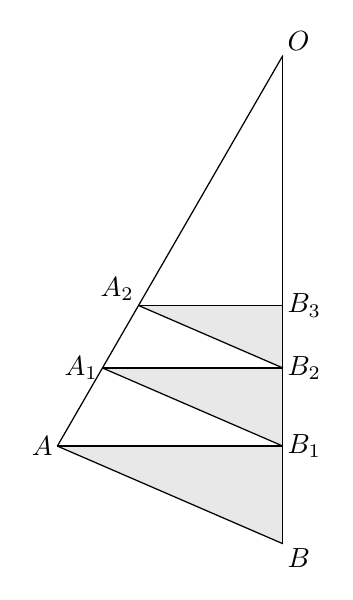
\begin{tikzpicture}[scale=0.62, line width=0.45pt,
  every node/.style={inner sep=1.5pt}]
  % OB 竖直（长 10），OA=b=9.238、∠AOB=θ=30°，公比 k=b·cosθ/a=0.8
  \coordinate (O)  at (0,10);
  \coordinate (B)  at (0,0);
  \coordinate (A)  at (-4.619,2.0);
  \coordinate (B1) at (0,2.0);
  \coordinate (A1) at (-3.695,3.6);
  \coordinate (B2) at (0,3.6);
  \coordinate (A2) at (-2.956,4.88);
  \coordinate (B3) at (0,4.88);
  % 阴影三角形（自下而上依次为 S₁、S₂、S₃）
  \fill[gray!18] (A) -- (B) -- (B1) -- cycle;
  \fill[gray!18] (A1) -- (B1) -- (B2) -- cycle;
  \fill[gray!18] (A2) -- (B2) -- (B3) -- cycle;
  % 各边
  \draw (O) -- (B);
  \draw (O) -- (A);
  \draw (A) -- (B);
  \draw (A) -- (B1);
  \draw (A1) -- (B1);
  \draw (A1) -- (B2);
  \draw (A2) -- (B2);
  \draw (A2) -- (B3);
  % 顶点标注
  \node[anchor=south west] at (O)  {$O$};
  \node[anchor=north west] at (B)  {$B$};
  \node[anchor=east]       at (A)  {$A$};
  \node[anchor=east]       at (A1) {$A_1$};
  \node[anchor=south east] at (A2) {$A_2$};
  \node[anchor=west]       at (B1) {$B_1$};
  \node[anchor=west]       at (B2) {$B_2$};
  \node[anchor=west]       at (B3) {$B_3$};
\end{tikzpicture}
\end{center}
\nopagebreak[4]
\Needspace{4\baselineskip}
\textbf{解析}
\nopagebreak[4]
\begin{center}% 1982 年全国卷（文科）第 9 题：△AOB 中作 AB₁⊥OB、B₁A₁∥BA，再作 A₁B₂⊥OB、B₂A₂∥BA，如此无限作下去；图中 OB 画成竖直线，故垂线 AB₁、A₁B₂、A₂B₃ 为水平线，阴影自下而上依次为 △ABB₁、△A₁B₁B₂、△A₂B₂B₃（按源卷布局）
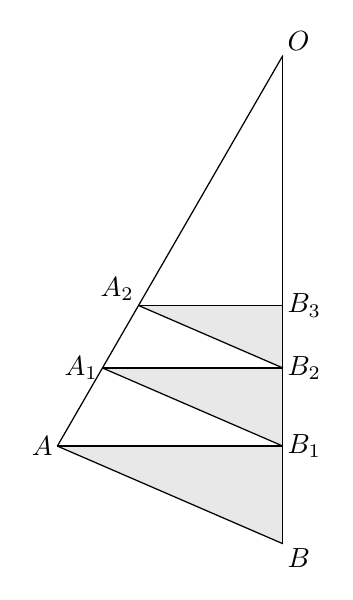
\begin{tikzpicture}[scale=0.62, line width=0.45pt,
  every node/.style={inner sep=1.5pt}]
  % OB 竖直（长 10），OA=b=9.238、∠AOB=θ=30°，公比 k=b·cosθ/a=0.8
  \coordinate (O)  at (0,10);
  \coordinate (B)  at (0,0);
  \coordinate (A)  at (-4.619,2.0);
  \coordinate (B1) at (0,2.0);
  \coordinate (A1) at (-3.695,3.6);
  \coordinate (B2) at (0,3.6);
  \coordinate (A2) at (-2.956,4.88);
  \coordinate (B3) at (0,4.88);
  % 阴影三角形（自下而上依次为 S₁、S₂、S₃）
  \fill[gray!18] (A) -- (B) -- (B1) -- cycle;
  \fill[gray!18] (A1) -- (B1) -- (B2) -- cycle;
  \fill[gray!18] (A2) -- (B2) -- (B3) -- cycle;
  % 各边
  \draw (O) -- (B);
  \draw (O) -- (A);
  \draw (A) -- (B);
  \draw (A) -- (B1);
  \draw (A1) -- (B1);
  \draw (A1) -- (B2);
  \draw (A2) -- (B2);
  \draw (A2) -- (B3);
  % 顶点标注
  \node[anchor=south west] at (O)  {$O$};
  \node[anchor=north west] at (B)  {$B$};
  \node[anchor=east]       at (A)  {$A$};
  \node[anchor=east]       at (A1) {$A_1$};
  \node[anchor=south east] at (A2) {$A_2$};
  \node[anchor=west]       at (B1) {$B_1$};
  \node[anchor=west]       at (B2) {$B_2$};
  \node[anchor=west]       at (B3) {$B_3$};
\end{tikzpicture}
\end{center}
\nopagebreak[4]
记 $OB=a$、$OA=b$、$\angle AOB=\theta$。

\Needspace{5\baselineskip}
\textbf{（i）求 $OB_1$。} $B_1$ 是 $A$ 在 $OB$ 上的垂足，在直角三角形中
\nopagebreak[4]
\[
OB_1=OA\cos\theta=b\cos\theta.
\]

\Needspace{5\baselineskip}
\textbf{（ii）公比。} $A_1B_1\parallel BA$，且 $O$、$A_1$、$A$ 共线、$O$、$B_1$、$B$ 共线，故
\nopagebreak[4]
\[
\triangle OA_1B_1\backsim\triangle OAB,
\]
\Needspace{5\baselineskip}
相似比
\nopagebreak[4]
\[
k=\frac{OB_1}{OB}=\frac{b\cos\theta}{a},
\]
\Needspace{5\baselineskip}
于是 $OA_1=k\cdot OA$、$A_1B_1=k\cdot AB$。因 $B_2$ 是 $A_1$ 在 $OB$ 上的垂足，
\nopagebreak[4]
\[
OB_2=OA_1\cos\theta=kb\cos\theta=k\cdot OB_1,
\]
即每一步都把 $OB_n$ 乘以同一个 $k$。故对一切 $n$，$\triangle OA_nB_n\backsim\triangle OAB$，相似比为 $k^n$。

\Needspace{5\baselineskip}
\textbf{（iii）面积成等比。} 三角形 $A_{n-1}B_{n-1}B_n$ 与 $ABB_1$ 的顶角相同，且
\nopagebreak[4]
\[
\frac{OA_{n-1}}{OA}=k^{\,n-1},\qquad
\frac{B_{n-1}B_n}{BB_1}=\frac{OB_{n-1}-OB_n}{OB-OB_1}=\frac{k^{\,n-1}(1-k)OB}{(1-k)OB}=k^{\,n-1},
\]
\Needspace{5\baselineskip}
所以
\nopagebreak[4]
\[
S_n=k^{2(n-1)}S_1,
\]
$\{S_n\}$ 是公比为 $k^2$ 的等比数列。

\Needspace{5\baselineskip}
\textbf{（iv）求 $S_1$。} $\triangle ABB_1$ 以 $OB$ 上的线段 $BB_1$ 为底，$A$ 到直线 $OB$ 的距离（即 $b\sin\theta$）为高，而
\nopagebreak[4]
\[
BB_1=OB-OB_1=a-b\cos\theta,
\]
\Needspace{5\baselineskip}
故
\nopagebreak[4]
\[
S_1=\frac12(a-b\cos\theta)\,b\sin\theta.
\]

\Needspace{5\baselineskip}
\textbf{（v）求和。} 因 $a\ge b$ 且 $\theta$ 为锐角，$k=\dfrac{b\cos\theta}{a}<1$（$a=b$ 且 $\theta=0$ 为退化情形），故 $k^2<1$，无穷级数收敛：
\nopagebreak[4]
\[
\sum_{n=1}^{\infty}S_n=\frac{S_1}{1-k^2}
=\frac{\frac12(a-b\cos\theta)b\sin\theta}{1-\dfrac{b^2\cos^2\theta}{a^2}}.
\]
\Needspace{5\baselineskip}
把分母通分：
\nopagebreak[4]
\[
1-\frac{b^2\cos^2\theta}{a^2}=\frac{a^2-b^2\cos^2\theta}{a^2}
=\frac{(a-b\cos\theta)(a+b\cos\theta)}{a^2},
\]
\Needspace{5\baselineskip}
与分子中的因子 $a-b\cos\theta$ 约去，得
\nopagebreak[4]
\[
\sum_{n=1}^{\infty}S_n=\frac12(a-b\cos\theta)b\sin\theta\cdot\frac{a^2}{(a-b\cos\theta)(a+b\cos\theta)}
=\frac{a^2b\sin\theta}{2(a+b\cos\theta)}.
\]

（等价写法：$\displaystyle\sum_{n=1}^{\infty}S_n=\frac{a}{a+b\cos\theta}\cdot\frac12ab\sin\theta$，即“$\triangle AOB$ 的面积乘以 $\dfrac{a}{a+b\cos\theta}$”。）

复算（数值）：取 $a=2$、$b=1$、$\theta=60^\circ$，则 $\cos\theta=\dfrac12$、$\sin\theta=\dfrac{\sqrt3}{2}$，$k=\dfrac{1\cdot\frac12}{2}=0.25$，$S_1=\dfrac12\left(2-\dfrac12\right)\cdot\dfrac{\sqrt3}{2}=\dfrac{3\sqrt3}{8}\approx0.6495$；级数和 $=\dfrac{0.6495}{1-0.0625}\approx0.6928$，而公式给出 $\dfrac{a^2b\sin\theta}{2(a+b\cos\theta)}=\dfrac{4\cdot\frac{\sqrt3}{2}}{2\times2.5}=\dfrac{2\sqrt3}{5}\approx0.6928$ 。再用逐项相加核对：$S_1+S_2+S_3+\cdots=0.6495\,(1+0.0625+0.0039+\cdots)\approx0.6495\times1.0667\approx0.6928$ 。

\gkanswer{答案：$\dfrac{a^2b\sin\theta}{2(a+b\cos\theta)}$}

\end{answer}